\chapter{Especificação de Requisitos} \label{cap:especificacao}

%%%%%%%%%%%%%%%%%%%%%%%%%%%%%%%%%%%%%%%%%%%%%%%%%%%%
%%%%%%%%%%%%%%%%%%%%%%%%%%%%%%%%%%%%%%%%%%%%%%%%%%%%

\section{Especificação da arquitetura do sistema}
\label{sec:requisitos_infra}

A arquitetura especificada neste trabalho define a organização técnica da solução proposta para comunicação, encaminhamento e persistência dos dados produzidos na rede de campo. Sua função é estruturar, de forma coerente, os componentes responsáveis pela coleta das informações, pela transição entre a comunicação embarcada e a infraestrutura de aplicação, e pelo armazenamento dos dados necessários ao funcionamento do sistema e às etapas posteriores de segurança e análise.

A solução foi organizada em quatro blocos principais: nós sensores e atuadores, gateway, backend/API e persistência. No trecho de campo, os nós realizam a coleta dos dados do ambiente e transmitem mensagens curtas por meio da arquitetura LoRaWAN, atendendo aos requisitos de operação em dispositivos com restrição energética e comunicação de baixo consumo. O gateway atua como elemento intermediário entre essa rede e a infraestrutura de aplicação, concentrando as funções de recepção, registro de metadados e encaminhamento das mensagens ao backend, em conformidade com os requisitos RF3 e RF6.

A partir do gateway, a comunicação passa a utilizar Wi-Fi e requisições HTTP, permitindo integrar a rede embarcada a uma API autenticada implantada em infraestrutura de nuvem e a um mecanismo centralizado de persistência. Essa organização busca manter a camada de aplicação disponível de forma contínua para o recebimento dos dados encaminhados pelo gateway, ao mesmo tempo em que facilita o armazenamento e a posterior utilização das informações coletadas.

Além dos dados de aplicação, como temperatura e luminosidade, a arquitetura prevê a persistência de metadados relevantes para o acompanhamento da comunicação, incluindo informações de origem, sequência, recepção e qualidade do enlace. Essa escolha atende aos requisitos RF5 e RF7, além de contribuir para a rastreabilidade da operação, conforme estabelecido em RNF6. A mesma base persistida também prepara a infraestrutura para a incorporação posterior de mecanismos de criptografia leve e de análise por aprendizado de máquina, em conformidade com RNF7 e RNF8.

A Figura~\ref{fig:arquitetura-especificada} apresenta a arquitetura técnica especificada para o sistema. A partir dessa organização, as subseções seguintes detalham os requisitos funcionais e não funcionais da infraestrutura proposta, que fundamentam e justificam as decisões arquiteturais adotadas.

\begin{figure}[htb]
  \caption{\label{fig:arquitetura-especificada}Arquitetura especificada do sistema proposto.}
  \begin{center}
      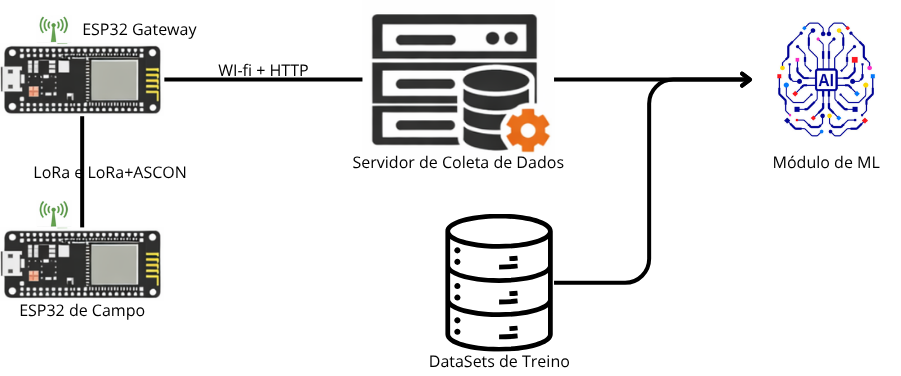
\includegraphics[scale=0.5]{figuras/arch_figure1.png}
  \end{center}

\end{figure}

%%%%%%%%%%%%%%%%%%%%%%%%%%%%%%%%%%%%%%%%%%%%%%%%%%%%

\subsection{Requisitos funcionais da infraestrutura proposta}

Os requisitos funcionais da infraestrutura proposta descrevem os comportamentos esperados da arquitetura do sistema, considerando a coleta, o encaminhamento, a autenticação e a persistência das informações produzidas na rede de campo.

\begin{enumerate}
    \item[RF1.] O sistema deve permitir que os nós de campo coletem e transmitam dados de aplicação, incluindo, no protótipo previsto, informações de temperatura e luminosidade.

    \item[RF2.] Cada mensagem transmitida pelos nós deve conter, além dos dados de aplicação, informações mínimas de identificação e acompanhamento, incluindo identificador do dispositivo e contador de mensagens.

    \item[RF3.] O gateway deve receber as mensagens provenientes da rede de campo, registrar os metadados de recepção e encaminhar essas informações ao backend por meio de rede Wi-Fi e requisições HTTP.

    \item[RF4.] O backend deve autenticar as requisições enviadas pelo gateway, restringindo o recebimento de dados a dispositivos previamente autorizados.

    \item[RF5.] O sistema deve persistir os dados de aplicação recebidos dos nós juntamente com os metadados associados à comunicação.

    \item[RF6.] A infraestrutura deve permitir armazenamento temporário das mensagens no gateway em situações de indisponibilidade da conexão com o backend, com possibilidade de reenvio posterior.

    \item[RF7.] Os dados persistidos devem permanecer disponíveis para uso posterior pelas camadas de segurança e de análise por aprendizado de máquina.
\end{enumerate}

%%%%%%%%%%%%%%%%%%%%%%%%%%%%%%%%%%%%%%%%%%%%%%%%%%%%

\subsection{Requisitos não funcionais da infraestrutura proposta}

Os requisitos não funcionais da infraestrutura proposta descrevem propriedades de operação e restrições que devem ser observadas para que a solução seja compatível com o contexto de sistemas embarcados e Internet das Coisas. Para sua elicitação e organização, adotou-se como referência a norma ISO/IEC 25010, considerando principalmente características relacionadas à eficiência de desempenho, confiabilidade, compatibilidade, manutenibilidade e segurança.

\begin{enumerate}
    \item[RNF1.] A infraestrutura deve ser compatível com a operação de nós de campo com restrições de energia, priorizando baixo consumo no trecho embarcado da comunicação.

    \item[RNF2.] A comunicação do sistema deve ser orientada a evento, evitando transmissões contínuas desnecessárias entre os componentes.

    \item[RNF3.] A arquitetura deve manter separação clara entre a rede de campo, baseada em LoRaWAN, e a infraestrutura de aplicação, baseada em Wi-Fi e HTTP.

    \item[RNF4.] O protótipo deve preservar simplicidade de integração entre hardware, comunicação e backend, de modo a manter viável sua montagem e evolução no contexto do projeto.

    \item[RNF5.] A infraestrutura deve apresentar robustez básica a falhas temporárias de conectividade entre gateway e backend.

    \item[RNF6.] O sistema deve garantir rastreabilidade das mensagens recebidas, por meio do registro de dados e metadados que permitam identificar origem, sequência, instante de recepção e condições básicas do enlace.

    \item[RNF7.] A arquitetura deve ser compatível com a incorporação posterior de mecanismos de criptografia leve sem exigir reformulação completa da infraestrutura de comunicação.

    \item[RNF8.] A infraestrutura deve ser compatível com o uso posterior de técnicas de aprendizado de máquina aplicadas à análise do comportamento da rede e à detecção de anomalias.
\end{enumerate}

%%%%%%%%%%%%%%%%%%%%%%%%%%%%%%%%%%%%%%%%%%%%%%%%%%%%
%%%%%%%%%%%%%%%%%%%%%%%%%%%%%%%%%%%%%%%%%%%%%%%%%%%%

\section{Requisitos do Sistema de Detecção de Anomalias}
A incorporação de um modelo de aprendizado de máquina à arquitetura proposta 
introduz requisitos específicos, distintos dos requisitos de infraestrutura 
definidos na Seção~\ref{sec:requisitos_infra}. O modelo será treinado e 
avaliado em ambiente computacional convencional, utilizando os dados 
históricos do \textit{dataset} Tour Perret. A viabilidade de portabilidade 
da fase de inferência para o gateway é tratada como perspectiva de 
continuidade, conforme discutido na Seção~7.3.

%%%%%%%%%%%%%%%%%%%%%%%%%%%%%%%%%%%%%%%%%%%%%%%%%%%%

\subsection{Requisitos Funcionais}

\begin{enumerate}

    \item[RF1.] O sistema deve receber como entrada sequências temporais das 
    variáveis selecionadas, organizadas por dispositivo e ordenadas 
    cronologicamente.

    \item[RF2.] O sistema deve produzir previsões do comportamento esperado de 
    cada variável monitorada e calcular o resíduo entre valor previsto e 
    valor observado para cada instante de tempo.

    \item[RF3.] O sistema deve classificar cada observação como normal ou 
    potencialmente anômala, com base em um critério de limiarização definido 
    a partir do conjunto de validação.

    \item[RF4.] O sistema deve permitir comparação quantitativa entre as três 
    abordagens de modelagem (ARIMA, RNN, LSTM) através de métricas 
    padronizadas de qualidade de previsão e detecção.

\end{enumerate}


%%%%%%%%%%%%%%%%%%%%%%%%%%%%%%%%%%%%%%%%%%%%%%%%%%%%

\subsection{Requisitos Não Funcionais}

\begin{enumerate}

    \item[RNF1.] O treinamento deve ser realizado exclusivamente sobre dados que 
    representem operação normal da rede, sem contaminação por observações 
    potencialmente anômalas.

    \item[RNF2.] O processo de treinamento e avaliação deve ser reprodutível, com 
    registro das sementes de inicialização, hiperparâmetros e critérios de 
    seleção de ordem utilizados em cada modelo.

\end{enumerate}

Essa orientação fortalece a coerência do trabalho como um todo. Em vez de separar artificialmente a fase de modelagem da fase de implantação, o desenvolvimento já considera que a utilidade prática dos modelos depende de um equilíbrio entre eficácia de detecção e viabilidade de execução em dispositivos restritos. Assim, a implementação proposta dialoga diretamente com a etapa posterior de avaliação energética e computacional.

Sob essa perspectiva, a comparação entre modelos não deverá considerar apenas métricas tradicionais de desempenho, mas também aspectos como simplicidade estrutural, custo computacional, volume de memória.

%%%%%%%%%%%%%%%%%%%%%%%%%%%%%%%%%%%%%%%%%%%%%%%%%%%%
%%%%%%%%%%%%%%%%%%%%%%%%%%%%%%%%%%%%%%%%%%%%%%%%%%%%

\section{Requisitos de Segurança do Sistema criptográfico}
\subsection{Segurança do Ascon-AEAD128}
Para o uso seguro da cifra, este trabalho adota os requisitos operacionais especificados pelo NIST para o Ascon-AEAD128 \cite{nist800232}. Embora a implementação utilizada corresponda à variante Ascon-128a (versão 1.2), esses requisitos são adotados de forma conservadora como limites aplicáveis, uma vez que ambas as versões compartilham a mesma taxa de processamento e a mesma estrutura de permutação, enquanto suas diferenças introduzem apenas sobrecarga constante. O primeiro requisito trata da geração da chave criptográfica, que deve seguir os padrões descritos no documento SP 800-133r2 \citeonline{barker2020nist133}, no qual é estabelecida a seguinte operação:

\[
K = U \oplus V,
\]

em que $U$ é uma cadeia de bits extraída de um Gerador de Bits Aleatórios (RBG - \textit{Random Bit Generator}) aprovado, e $V$ consiste em uma sequência de bits gerada independentemente de $U$, podendo ser composta inteiramente por zeros.

As especificações para os geradores de bits aleatórios aprovados estão descritas no documento SP 800-90A \citeonline{barker2015nist90a}. Neste projeto, será utilizado um Gerador Determinístico de Bits Aleatórios (DRBG - \textit{Deterministic Random Bit Generator}) através do mecanismo CTR\_DRBG. Essa escolha justifica-se pelo fato de que a entropia bruta extraída diretamente do hardware pode conter vícios físicos, tornando indispensável um estágio secundário de tratamento e condicionamento algorítmico \cite{turan2018nist90b}. Dessa forma, a implementação fará uso da biblioteca nativa \textit{mbedTLS} do ESP32, que extrai a entropia verdadeira do periférico de hardware (TRNG) e a processa através do algoritmo CTR\_DRBG, garantindo uma saída perfeitamente balanceada para a geração da chave.

Com base nesses elementos, os requisitos de segurança do Ascon-AEAD128 podem ser organizados em requisitos funcionais e não funcionais.

\subsubsection{Requisitos funcionais}

\begin{enumerate}
    \item[RF1.] A implementação da biblioteca \textit{ascon-suite} deve ser validada previamente, conforme discutido na Seção \ref{subsec:validacao-ascon}.

    \item[RF2.] A geração da chave criptográfica deve seguir os padrões descritos no documento SP 800-133r2 \citeonline{barker2020nist133}, adotando a operação $K = U \oplus V$.

    \item[RF3.] O sistema deve utilizar um Gerador Determinístico de Bits Aleatórios (DRBG - \textit{Deterministic Random Bit Generator}) através do mecanismo CTR\_DRBG para a geração de chaves criptográficas.

    \item[RF4.] A implementação deve fazer uso da biblioteca nativa \textit{mbedTLS} do ESP32 para extrair a entropia verdadeira do periférico de hardware (TRNG) e processá-la através do algoritmo CTR\_DRBG.

    \item[RF5.] Caso a renovação da chave simétrica se faça necessária por eventuais comprometimentos ou políticas de segurança, o sistema deve adotar o método de encapsulamento de chaves (\textit{key wrapping}), utilizando a chave secreta atual, desde que ainda válida e segura, para cifrar a nova chave gerada e permitir seu compartilhamento e atualização de forma segura entre o dispositivo e o nó de borda (\textit{Edge}).
\end{enumerate}

\subsubsection{Requisitos não funcionais}

\begin{enumerate}
    \item[RNF1.] A entropia bruta extraída diretamente do hardware não deve ser utilizada sem tratamento adicional, uma vez que pode conter vícios físicos (\textit{bias}), tornando indispensável um estágio secundário de condicionamento algorítmico \cite{turan2018nist90b}.

    \item[RNF2.] A chave criptográfica deve ser mantida em sigilo absoluto, aliada à garantia de unicidade do \textit{nonce} para cada operação de encriptação.

    \item[RNF3.] Para \textit{tags} de autenticação cujo tamanho $\lambda$ (em bits) satisfaça a condição $64 \leq \lambda \leq 128$, a quantidade de falhas de decriptação não deve exceder $2^{\lambda - 32}$.

    \item[RNF4.] O volume máximo de dados processados durante as rotinas de encriptação e decriptação não deve ultrapassar $2^{54}$ bytes para uma mesma chave, devendo a chave ser obrigatoriamente renovada caso esse limite seja atingido.
\end{enumerate}

Diante desses requisitos, alguns deles possuem impacto prático reduzido no contexto deste projeto. Como as redes LoRaWAN operam com taxas de transmissão extremamente baixas e pacotes pequenos, atingir o limite de $2^{54}$ bytes processados sob uma mesma chave é inviável durante a vida útil física do dispositivo. Da mesma forma, considerando o uso de uma \textit{tag} de 128 bits, o limite tolerado antes da obrigatoriedade de rotação da chave é de $2^{96}$ falhas de decriptação. Alcançar esse volume de tentativas de ataques de injeção na rede é improvável, dadas as severas restrições de tempo de transmissão inerentes ao protocolo.
